\documentclass{article}
\usepackage[T1]{fontenc}
\usepackage{lmodern}
\usepackage{graphicx}
\usepackage{amsmath,amssymb}
\usepackage[a4paper,margin=2cm]{geometry}
\usepackage[absolute,overlay]{textpos}
\setlength{\TPHorizModule}{1mm}
\setlength{\TPVertModule}{1mm}
\usepackage[indonesian]{babel}
\usepackage{hyperref}
\setlength{\emergencystretch}{2em}
% unit: Halaman 36

\begin{document}

% === Halaman 36 (llm) ===

\vspace{234.63mm}

\section*{Forward Mixing and Backward Mixing}\vspace{10mm}

% deskripsi: Diagram skema proses Forward Mixing dan Backward Mixing pada algoritma kriptografi, menunjukkan aliran data melalui S-boxes, rotasi, penambahan kunci (K), dan operasi XOR.
% bbox normalisasi: [0.0700, 0.1000, 0.8500, 0.8900]
\begin{textblock*}{163.80mm}(14.70mm,29.70mm)
\noindent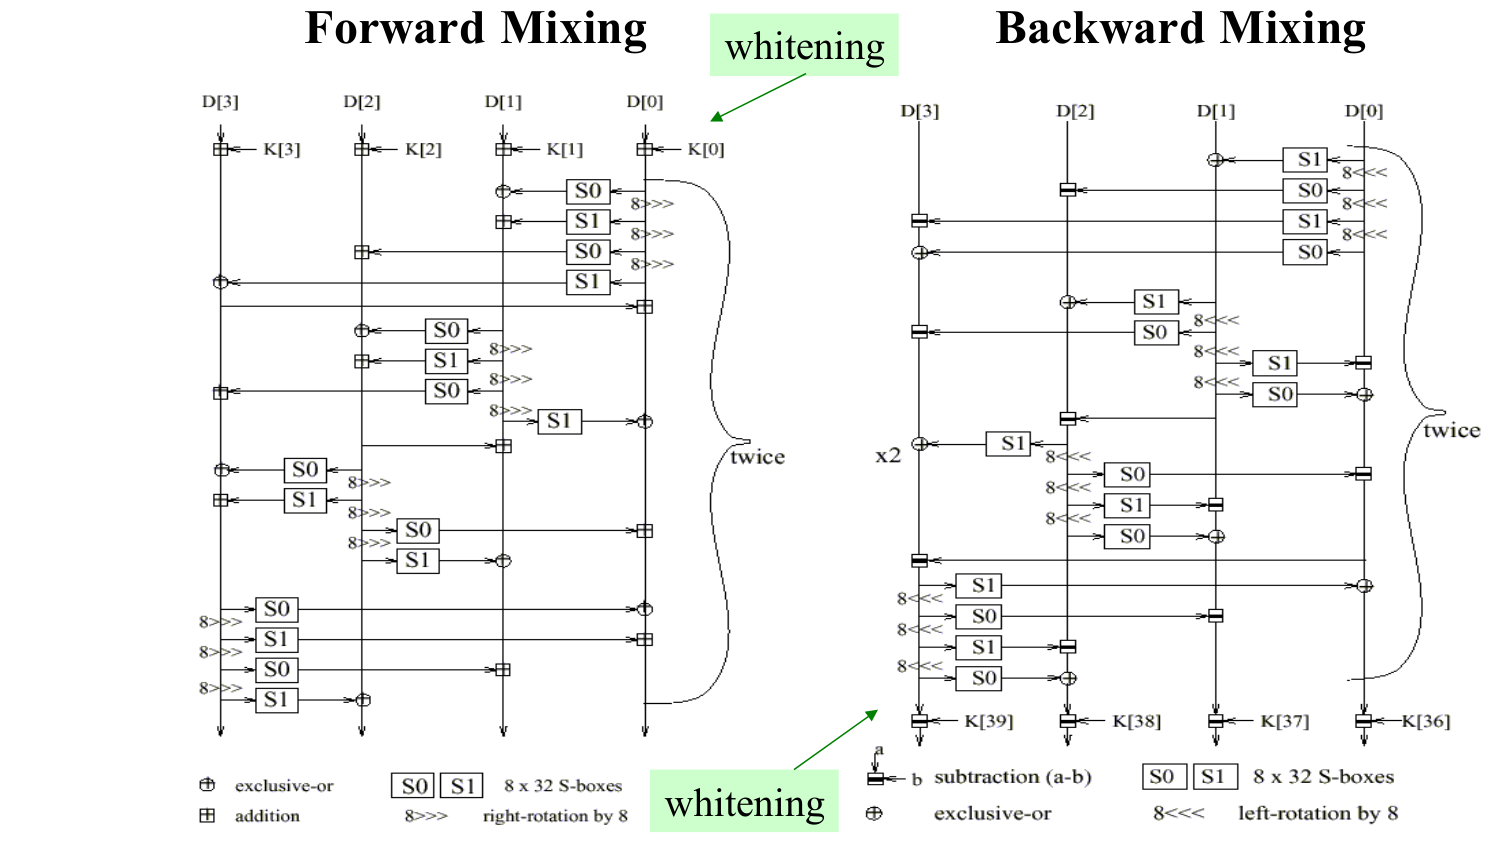
\includegraphics[width=163.80mm,height=234.63mm]{../../images/llm/page_036_img_01.png}%
\end{textblock*}

\end{document}
